%%%%%%%%%%%%%%%%%%%%%%%%%%%%%%%%%%%%%%%%%%%%%%%%%%%%
% This will help you in writing your homebook
% Remember that the character % is a comment in latex
%
% chapter 1
\chapter{Prototype}
\label{chap1}
\graphicspath{ {./chapters/chap1images/} }
%%%%%%%%%%%%%%%%%%%%%%%%%%%%%%%%%%%%%%%%%%%%%%%%%%%%%%%%%%%
% you can organize a chapter using sections -> \section{Simulating an inverter}
% or subsections -> \subsection{simulating a particular type of inverter}
%%%%%%   First section
\section{Introduction}
In order to better and easier simulate the architecture, two scripts have been used:
A bash script to control the simulation from high level: it is in charge to invoke the C script with the right command line argument during the proper simulation phase and to 
run modelsim;
A C script in charge to perfrom various operations during different steps of the simulation, manipulating different files.
For simplicity, a single value is assigned to both operands each simulation cycle, de facto using the multiplier as a square-evaluation circuit.
\section{General simulation flow}
The C script can accepts an additional command line parameter:\begin{itemize}
    \item -i corresponds to \textbf{TEST\_INIT} mode: the script reads the handwrittensamples.txt file, in which desired inputs in human-like format are stored, e.g. 12.29487, -0.9872 etc, 
    and generates two other files as output, both storing data in hexadecimal encoding:
    simulationinputs.hex, which contains the inputs for the Modlesim simulation
    expected\_outputs.hex, which contains the outputs that are expected to be generated by the Modelsim simulation.
    \item -v corresponds to \textbf{TEST\_VALIDATION} mode: the script executes a diff command between the self-generated expected\_outputs.hex file and the file generated by the Modelsim simulation using 
    a pipe to execute it in background and take back its output, then processing it in order to establish if the two files are identical, Test Successful, or different, Test Failed.
    
    \end{itemize} 

The flow of the simulation is the following:
\begin{enumerate}
    \item the bash script executes the C program passing -i as command line parameter in order to generate the input vectors for the simulation and the file storing the expected results.
    \item Modelsim is launched and the effective output file is generated
    \item the C program is executed passing -v as command line parameter in order to compare the simulation results with the expected ones
    \end{enumerate} 

    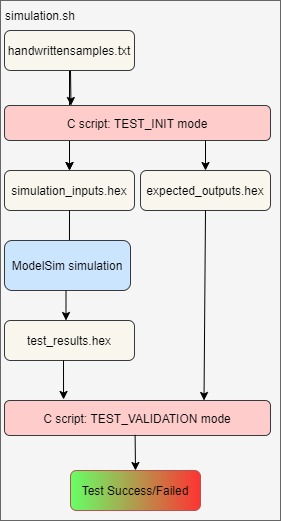
\includegraphics[height=12cm]{{./schematic/lab2_SimulationFlow.jpg}}
\section{C script - Key Aspects}
Since IEEE754 is the standard encoding that is normally used to store floating point data inside a flash memory, to convert a floating point value in its equivalent hexadecimal 
encoding it's sufficient to use the   \textbf{union}  C data type.
\textbf{union} data type allows to store multiple-encoding data variables in the same memory location, thus it is sufficient read a value from the handwrittensamples.hex file 
and store it as a float variable inside the previously declared memory location, and then accessing it as a 32-bit data variable, using the C standard type \textbf{uint32\_t}.
\begin{lstlisting}[style=CStyle]
    union IEEE754conv 
    {
        float f;
        uint32_t ieee754Value;
    };

\end{lstlisting}

The previously described operation is trivially implemented by the following procedure, that is very convenient both in terms synthax and in terms of CPU time, since what is done is just a couple of memory accesses:
\begin{lstlisting}[style=CStyle]
    uint32_t convFloatinIEEE754(float val)
    {
            union IEEE754conv conv;
            conv.f = val;
            return conv.ieee754Value;
    }
\end{lstlisting}
\section{Simulation Results}
Simulating the architecture with the procedure described above, it has been confirmed that it behaves in the expected way, since the results it produces are coincident with
the expected ones generated by the C script.
Tests have been made with both positive and negative numbers, with different orders of magnitudes for the modules, on both Ubuntu and Centos Linux OS. In case a new simulation has to be performed on a different Linux system, a bash script, compile.bash, is provided in order to 
quickly recompile binaries.
